\section{Numerische Lösung nicht linearer Gleichungssysteme}

\begin{remark}
    LGS = lineares Gleichungssystem, NGS = nichtlineares Gleichungssystem
\end{remark}



\raggedcolumns

\begin{definition}{Skalarwertige Funktionen}
    $f: D \subset \R^n \to W \subset \R$
    \vspace{-2mm}
    $$(x_1, x_2, \ldots, x_n) \mapsto y = f(x_1, x_2, \ldots, x_n)$$
    \small
    $f$ mit $n$ unabhängigen Variablen $x_1, \ldots, x_n$ und einer abhängigen Variablen $y$,
    die jedem $(x_1, x_2, \ldots, x_n)$ aus Definitionsmenge $D \subset \R^n$ genau ein $y \in W \subset \R$ zuordnet.
    Ergebnis: $y \in \R$ = Skalar (eine Zahl) 
\end{definition}

\begin{concept}{Vektorwertige Funktion} gibt einen \textbf{Vektor} zurück (statt Skalar)\\
    Sei $\textbf{f}: \R^n \to \R^m$ eine Funktion mit $n$ Variablen.
    \vspace{-2mm}
    $$\textbf{f}(x_1 \ldots, x_n) = \begin{psmallmatrix} y_1 = f_1(x_1, x_2, \ldots, x_n) \\ y_2 = f_2(x_1, x_2, \ldots, x_n) \\ ... \\ y_m = f_m(x_1, x_2, \ldots, x_n) \end{psmallmatrix}$$
    \small wobei die $m$ Komponenten $f_i: \R^n \to \R$ für $i = 1, 2, \ldots, n$ von $\textbf{f}$ wieder \textbf{skalarwertige} Funktionen sind.
\end{concept}

\begin{theorem}{Nichtlineares Gleichungssystem (NGS)}\\
    Lösungen des NGS sind Nullstellen der Funktion:
    \vspace{-2mm}
    $$\textbf{f}: \R^2 \to \R^2 \quad \textbf{f}(x) = \begin{psmallmatrix} f_1 (x_1, x_2) \\ f_2 (x_1, x_2) \end{psmallmatrix} = \begin{psmallmatrix} 0\\ 0 \end{psmallmatrix}$$
    \small
    Ein solches System lässt sich nicht in die Form $Ax = b$ bringen. \\
    Geometrisch lassen sich die Lösungen als Schnittpunkte der beiden Funktionen interpretieren.
\end{theorem}

\begin{corollary}{Lineare Funktionen von LGS}
    $$\textbf{A} \overrightarrow{\textbf{x}} = \overrightarrow{\textbf{b}} \Rightarrow \underbrace{\textbf{A} \overrightarrow{\textbf{x}} - \overrightarrow{\textbf{b}} = \overrightarrow{\textbf{0}}}_{\overrightarrow{\textbf{f}}(\overrightarrow{\textbf{x}})} \Rightarrow \overrightarrow{\textbf{f}}(x_1, x_2, x_3) = 0 \begin{psmallmatrix} x_1 \\ x_2 \\ x_3 \end{psmallmatrix} = \begin{psmallmatrix} 0 \\ 0 \\ 0 \end{psmallmatrix}$$
    \resizebox{\textwidth}{!}{
    $\overrightarrow{\textbf{f}}(\overrightarrow{\textbf{x}}) = \textbf{A} \overrightarrow{\textbf{x}} - \overrightarrow{\textbf{b}} = \begin{psmallmatrix} 4 & -1 & 1 \\ -2 & 5 & 1 \\ 1 & -2 & 5 \end{psmallmatrix} \begin{psmallmatrix} x_1 \\ x_2 \\ x_3 \end{psmallmatrix} - \begin{psmallmatrix} 5 \\ 11 \\ 12 \end{psmallmatrix}, \quad
    \textbf{f}(x_1, x_2, x_3) = \begin{psmallmatrix} f_1 = 4x_1 - x_2 + x_3 - 5 \\ f_2 = -2x_1 + 5x_2 + x_3 - 11 \\ f_3 = x_1 - 2x_2 + 5x_3 - 12 \end{psmallmatrix}$}
\end{corollary}


\begin{concept}{Analytische Darstellung}
    \begin{itemize}
        \item \textbf{Explizite Darstellung:} $y = f(x_1, \ldots, x_n)$
        \item \textbf{Implizite Darstellung:} $F(x, y) = 0$
        \item \textbf{Parameterdarstellung:} $x = x(t), y = y(t)$
    \end{itemize}
\end{concept}

\begin{concept}{Darstellung durch Wertetabelle}
    Sei $f: \R^n \to \R^m$ eine Funktion.\\
    In $z = f(x,y)$ Werte von $x$ und $y$ einsetzen (der Reihe nach): \\
    $$\begin{psmallmatrix} z_{11} & z_{12} & \ldots & z_{1m} \\ z_{m1} & z_{m2} & \ldots & z_{mn} \end{psmallmatrix} \quad\quad\quad\quad\quad\quad\quad\quad\quad\quad\quad\quad\quad\quad.$$
\end{concept}

\begin{minipage}{0.5\linewidth}
\begin{concept}{Funktion als Fläche im Raum}\\
    $f$ ordnet jedem Punkt $(x, y) \in D$ in Ebene Wert $z=f(x, y)$ zu \\($\rightarrow$ Höhenkoordinate)    
\end{concept}

\begin{concept}{Schnittkurvendiagramm}\\
    Fläche $z=f(x, y)$ bei konstanten Höhe $z$ schneiden: Schnittkurve. 
    Diese in $(x, y)$-Ebene projizieren: Höhenlinie.
\end{concept}
\end{minipage}
\begin{minipage}{0.5\linewidth}
\vspace{-8mm}
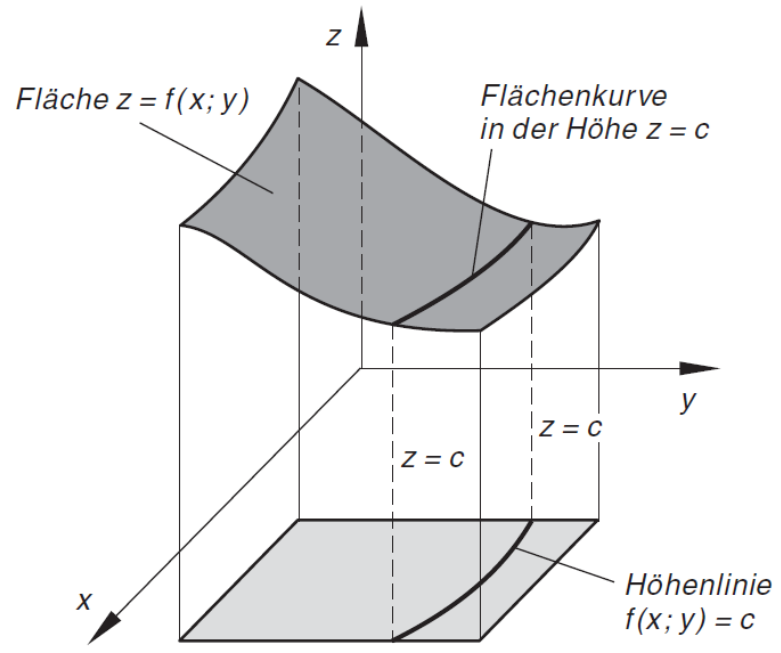
\includegraphics[width=\linewidth]{grafische_darstellung_detailed.png}
\small hellgraue Fläche = Definitionsbereich D
\end{minipage}

\subsubsection{Partielle Ableitungen}

\begin{theorem}{Partielle Ableitung}
$
f^{\prime}(x_0)=\lim _{\Delta x \rightarrow 0} \frac{(f(x_0+\Delta x)-f(x_0))}{\Delta x}
$
$$\text{Ableitung nach x: } f_x=\frac{\partial f}{\partial x}(x, y)=\lim _{\Delta x \rightarrow 0} \frac{f(x+\Delta x, y)-f(x, y)}{\Delta x}$$
$$\text{Ableitung nach y: } f_y=\frac{\partial f}{\partial y}(x, y)=\lim _{\Delta y \rightarrow 0} \frac{f(x, y+\Delta y)-f(x, y)}{\Delta y}$$
\end{theorem}



\begin{KR}{Partielle Ableitungen berechnen}
    \small
    \begin{enumerate}
        \item Variable identifizieren: nach welcher Variable ableiten?
        \item Alle anderen Variablen während Ableitung nur Konstanten
        \item Standardableitungsregeln anwenden und Ergebnis korrekt notieren
    \end{enumerate}
\end{KR}

\begin{definition}{Jacobi-Matrix}
    \resizebox{0.7\textwidth}{!}{
$f: \mathbb{R}^n \rightarrow \mathbb{R}^m$ mit $y = f(x)$ und $x = (x_1, x_2, ..., x_n)^T \in \mathbb{R}^n$}

Jacobi-Matrix enthält alle partiellen Ableitungen 1. Ordnung von $f$:
\vspace{-2mm}\\
$$f(x) = \begin{psmallmatrix}
    y_1=f_1(x) \\
    y_2=f_2(x) \\
    ...\\
    y_m=f_m(x)
\end{psmallmatrix} \rightarrow 
Df(x) := \begin{bsmallmatrix}
\frac{\partial f_1}{\partial x_1}(x) & \frac{\partial f_1}{\partial x_2}(x) & \cdots & \frac{\partial f_1}{\partial x_n}(x) \\
\frac{\partial f_2}{\partial x_1}(x) & \frac{\partial f_2}{\partial x_2}(x) & \cdots & \frac{\partial f_2}{\partial x_n}(x) \\
\cdots & \cdots & \cdots & \cdots \\
\frac{\partial f_m}{\partial x_1}(x) & \frac{\partial f_m}{\partial x_2}(x) & \cdots & \frac{\partial f_m}{\partial x_n}(x)
\end{bsmallmatrix}$$
\end{definition}

\begin{concept}{Linearisierung}
Die verallgemeinerte \textcolor{purple}{\textbf{Tangentengleichung}}
$$g(x) = f(x^{(0)}) + Df(x^{(0)}) \cdot (x - x^{(0)})$$ 
\small
beschreibt lineare Funktion, $f(x) \approx g(x)$ in Umgebung von $x^{(0)}=(x_1^{(0)}, x_2^{(0)}, \ldots, x_n^{(0)})^T \in \mathbb{R}^n$. 
Man spricht von der \textbf{Linearisierung} der Funktion $y = f(x)$ in einer Umgebung von $x^{(0)}$ ($x^{(k)}$ bezeichnet Vektor aus $\R^n$ nach $k$-ter Iteration).
\end{concept}

\begin{corollary}{Tangentialebene}
    \resizebox{0.7\textwidth}{!}{
    $f: \mathbb{R}^2 \longrightarrow \mathbb{R}$, $y=f(x_1, x_2)$, $\boldsymbol{x}^{(0)}=(x_1^{(0)}, x_2^{(0)})^T \in \mathbb{R}^2$ }

    Spezielle Jacobi-Matrix (nur ein Zeilenvektor mit zwei Elementen):
    $$Df(x^{(0)}) = \left(\frac{\partial f}{\partial x_1}(x_1^{(0)}, x_2^{(0)}), \frac{\partial f}{\partial x_2}(x_1^{(0)}, x_2^{(0)})\right)$$
    Linearisierung $g(x_1, x_2)$ die Gleichung der Tangentialebene: 
    $$=f(x_1^{(0)}, x_2^{(0)}) + \left(\frac{\partial f}{\partial x_1}(x_1^{(0)}, x_2^{(0)}), \frac{\partial f}{\partial x_2}(x_1^{(0)}, x_2^{(0)})\right) \cdot \binom{x_1 - x_1^{(0)}}{x_2 - x_2^{(0)}}$$
    $$= f(x_1^{(0)}, x_2^{(0)}) + \frac{\partial f}{\partial x_1}(x_1^{(0)}, x_2^{(0)}) \cdot (x_1 - x_1^{(0)}) + \frac{\partial f}{\partial x_2}(x_1^{(0)}, x_2^{(0)}) \cdot (x_2 - x_2^{(0)})$$
    \small
    Sie enthält sämtliche im Flächenpunkt 
    $\stackrel{\bullet}{P}=\left(x_1^{(0)}, x_2^{(0)}, f(x_1^{(0)}, x_2^{(0)})\right)$ \\
    an die Bildfläche von $y=f(x_1, x_2)$ angelegten Tangenten.
\end{corollary}

\begin{KR}{Jacobi-Matrix berechnen und linearisieren}\\
Sei $f: \mathbb{R}^n \rightarrow \mathbb{R}^m$ mit $y = f(x)$ und $x = (x_1, x_2, ..., x_n)^T \in \mathbb{R}^n$. 
\vspace{-2mm}\\
\begin{enumerate}
    \item Identifiziere die Komponentenfunktionen $f_1, f_2, ..., f_m$ und \\ Variablen $x_1, x_2, ..., x_n$.
    \item Berechne partielle Ableitungen $\frac{\partial f_i}{\partial x_j}$ für $i = 1, ..., m$, $j = 1, ..., n$.
    \item Stelle die Jacobi-Matrix $Df(x)$ auf
    \item Werte Jacobi-Matrix an Entwicklungspunkt $x^{(0)}$ aus\\ (Werte für $x_1, x_2, ..., x_n$ einsetzen)
    \item Berechne Linearisierung $g(x)$ mit Tangentengleichung
\end{enumerate}
\end{KR}

\begin{example2}{Jacobi-Matrix und Linearisierung}
$f(x, y, z) = \begin{psmallmatrix} e^{xy} + z^2 - 3 \\ \sin(x + y) - z \\ x^2 + y^2 + z^2 - 6 \end{psmallmatrix}$

\textbf{Jacobi-Matrix:}
$Df(x, y, z) = \begin{bsmallmatrix} ye^{xy} & xe^{xy} & 2z \\ \cos(x + y) & \cos(x + y) & -1 \\ 2x & 2y & 2z \end{bsmallmatrix}$

\textbf{Linearisierung an $(1, 0, 1)^T$:}

\resizebox{\textwidth}{!}{
$f(1, 0, 1) = \begin{psmallmatrix} e^0 + 1 - 3 \\ \sin(1) - 1 \\ 1 + 0 + 1 - 6 \end{psmallmatrix} = \begin{psmallmatrix} -1 \\ \sin(1) - 1 \\ -4 \end{psmallmatrix}, \quad
Df(1, 0, 1) = \begin{bsmallmatrix} 0 & 1 & 2 \\ \cos(1) & \cos(1) & -1 \\ 2 & 0 & 2 \end{bsmallmatrix}$}

Linearisierung: $g(x, y, z) = f(1, 0, 1) + Df(1, 0, 1) \cdot \begin{psmallmatrix} x - 1 \\ y - 0 \\ z - 1 \end{psmallmatrix}$

$$g(x, y, z) = \begin{psmallmatrix} -1 + y + 2(z-1) \\ \sin(1) - 1 + \cos(1)(x-1) + \cos(1)y - (z-1) \\ -4 + 2(x-1) + 2(z-1) \end{psmallmatrix}$$

\textbf{Geometrische Bedeutung:}
Die Linearisierung approximiert die nichtlineare Funktion $f$ in der Nähe des Punktes $(1, 0, 1)^T$ durch eine lineare Funktion. Dies entspricht der Tangentialebene an die durch $f = 0$ definierte Fläche im dreidimensionalen Raum.
\end{example2}

\raggedcolumns

\subsubsection{Nullstellenbestimmung für NGS}

\begin{definition}{Problemstellung zur Nullstellenbestimmung}\\
Gegeben sei $n \in \mathbb{N}$ und eine Funktion $f: \mathbb{R}^n \rightarrow \mathbb{R}^n$. Gesucht ist ein Vektor $\bar{x} \in \mathbb{R}^n$ mit $f(\bar{x}) = 0$.

Komponentenweise bedeutet dies: Gegeben sind $n$ Funktionen $f_i: \mathbb{R}^n \rightarrow \mathbb{R}$, die die Komponenten von $f$ bilden. Gesucht ist ein Vektor $\bar{x} \in \mathbb{R}^n$ mit $f_i(\bar{x}) = 0$ für $i = 1, ..., n$.
\end{definition}

\begin{concept}{Quadratisch konvergentes Newton-Verfahren} \small{(Quadratische Konv.)}\\
    \normalsize
    Gesucht sind Nullstellen von $f: \mathbb{R}^n \rightarrow \mathbb{R}^n$. Sei $x^{(0)}$ ein Startvektor in der Nähe einer Nullstelle. 
    Das Newton-Verfahren zur näherungsweisen Bestimmung dieser Nullstelle lautet:

    Lösung von $f(x)=0$ mit $f: \mathbb{R}^n \rightarrow \mathbb{R}^n$ für $n=0,1,2, \ldots$
    \begin{enumerate}
        \item Berechne $f(x^{(n)})$ und $D f(x^{(n)})$
        \item Berechne $\delta^{(n)}$ als Lösung des linearen Gleichungssystems
        $$Df(x^{(n)}) \cdot \delta^{(n)} = -f(x^{(n)})$$
        \item Setze $x^{(n+1)} := x^{(n)} + \delta^{(n)}$
    \end{enumerate}
\end{concept}

\begin{theorem}{Vereinfachtes Newton-Verfahren} (Lineare Konvergenz)

    Lösung von $f(x)=0$ mit $f: \mathbb{R}^n \rightarrow \mathbb{R}^n$ für $n=0,1,2, \ldots$
    \begin{enumerate}
        \item Berechne $f(x^{(n)})$ und $D f(x^{(0)})$
        \item Berechne $\delta^{(n)}$ als Lösung des lin. GS $D f\left(x^{(0)}\right) \cdot \delta^{(n)}=-f\left(x^{(n)}\right)$
        \item Setze $x^{(n+1)}:=x^{(n)}+\delta^{(n)}$
    \end{enumerate}
\end{theorem}

\begin{KR}{Newton-Verfahren für nichtlineare Gleichungssysteme}
\paragraph{Schritt 1: Funktionen und Jacobi-Matrix aufstellen}
Definiere $f(x) = 0$ und berechne die Jacobi-Matrix $Df(x)$.

\paragraph{Schritt 2: Startvektor wählen}
Wähle einen geeigneten Startvektor $x^{(0)}$ nahe der vermuteten Lösung.

\paragraph{Schritt 3: Iterative Berechnung}
Für jede Iteration $k$:
\begin{itemize}
    \item \textbf{Linearisierung um} $x^{(k)}$: Berechne $f(x^{(k)})$ und $Df(x^{(k)})$
    \item \textbf{Nullstelle der Linearisierung berechnen}: \\ Löse das LGS: $Df(x^{(k)}) \delta^{(k)} = -f(x^{(k)})$
    \item \textbf{Nächste Iteration}: Setze $x^{(k+1)} = x^{(k)} + \delta^{(k)}$
\end{itemize}
\vspace{2mm}
\textbf{Formel:}
        $x^{(k+1)}=x^{(k)}-(D f(x^{(k)}))^{-1} \cdot f(x^{(k)})$
\paragraph{Schritt 4: Konvergenzprüfung}
Prüfe Abbruchkriterien wie $$\|f(x^{(k+1)})\|_2 < \text{TOL} \text{ oder } \|x^{(k+1)} - x^{(k)}\|_2 < \text{TOL}$$

\paragraph{Schritt 5: Lösung interpretieren}
Die konvergierte Lösung $x^{(k)}$ ist eine Näherung für die Nullstelle.
\end{KR}

\begin{example2}{Newton-Verfahren anwenden} Löse das Gleichungssystem 
$$f(x_1, x_2) = \begin{psmallmatrix} 20 - 18x_1 - 2x_2^2 \\ -4x_2(x_1 - x_2^2) \end{psmallmatrix} = \begin{psmallmatrix} 0 \\ 0 \end{psmallmatrix}$$
mit dem Newton-Verfahren für den Startvektor $x^{(0)} = (1.1, 0.9)^T$.
\vspace{2mm}\\
\textbf{Schritt 1:} Jacobi-Matrix berechnen
$$Df(x_1, x_2) = \begin{bsmallmatrix} -18 & -4x_2 \\ -4x_2 & -4(x_1 - 3x_2^2) \end{bsmallmatrix}$$

\textbf{Schritt 2:} Erste Iteration ($k = 0$)
$$f(1.1, 0.9) = \begin{psmallmatrix} -1.42 \\ -0.036 \end{psmallmatrix}$$
$$Df(1.1, 0.9) = \begin{bsmallmatrix} -18 & -3.6 \\ -3.6 & -5.32 \end{bsmallmatrix}$$

LGS lösen: $\begin{bsmallmatrix} -18 & -3.6 \\ -3.6 & -5.32 \end{bsmallmatrix} \delta^{(0)} = \begin{psmallmatrix} 1.42 \\ 0.036 \end{psmallmatrix}$
$\Rightarrow \delta^{(0)} = \begin{psmallmatrix} -0.0822 \\ 0.0178 \end{psmallmatrix}$
$$x^{(1)} = \begin{psmallmatrix} 1.1 \\ 0.9 \end{psmallmatrix} + \begin{psmallmatrix} -0.0822 \\ 0.0178 \end{psmallmatrix} = \begin{psmallmatrix} 1.0178 \\ 0.9178 \end{psmallmatrix}$$

Weitere Iterationen führen zur Konvergenz.
\end{example2}

\begin{example2}{Beispiel mit Newton-Verfahren}
    
Gegeben sind zwei Gleichungen und der Start-Vektor $x^{(0)}=(2,-1)^T$

$$
1-x^2=y^2, \quad \frac{(x-2)^2}{a}+\frac{(y-1)^2}{b}=1
$$


Umwandlung in Funktionen $f_1, f_2=0$

$$
f_1(x, y)=1-x^2-y^2=0, \quad f_2(x, y)=\frac{(x-2)^2}{a}+\frac{(y-1)^2}{b}-1=0
$$


Vektorwertige Funktion und Jacobi-Matrix bilden

$$
D f(x, y)=\left(\begin{array}{cc}
-2 x & -2 y \\
\frac{2 x-4}{a} & \frac{2 y-2}{b}
\end{array}\right), \quad f(x, y)=\binom{1-x^2-y^2}{\frac{(x-2)^2}{a}+\frac{(y-1)^2}{b}-1}
$$


Start-Vektor $x^{(0)}$ einsetzen

$$
D f(2,-1)=\left(\begin{array}{cc}
-4 & 2 \\
0 & -4 / b
\end{array}\right), \quad f(2,-1)=\binom{-4}{4 / b-1}
$$


Berechne $\delta^{(0)}$

$$
\left(D f\left(x^{(0)}\right) \mid-f\left(x^{(0)}\right)\right)=\left(\begin{array}{cc|c}
-4 & 2 & 4 \\
0 & -4 / b & -4 / b+1
\end{array}\right) \rightarrow \underbrace{\binom{-1}{0}}_{\delta^{(0)}}
$$


Berechne $x^{(1)}$

$$
x^{(1)}=\underbrace{\binom{2}{-1}}_{x^{(0)}}+\underbrace{\binom{-1}{0}}_{\delta^{(0)}}=\binom{1}{-1}
$$
\end{example2}

\subsection{Gedämpftes Newton-Verfahren}

\begin{corollary}{Gedämpftes Newton-Verfahren}

Nur in der Nähe der Nullstelle ist Konvergenz des Verfahrens garantiert!
\begin{enumerate}
    \item Berechne $f\left(x^{(n)}\right)$ und $D f\left(x^{(n)}\right)$
    \item Berechne $\delta^{(n)}$ als Lösung des lin. GS $D f\left(x^{(n)}\right) \cdot \delta^{(n)}=-f\left(x^{(n)}\right)$
    \item Finde das minimale $k \in\left\{0,1, \ldots, k_{\max }\right\}$ mit:
\end{enumerate}
$$
\left\|f\left(x^{(n)}+\frac{\delta^{(n)}}{2^k}\right)\right\|_2<\left\|f\left(x^{(n)}\right)\right\|_2
$$
Kein minimales $k$ gefunden $\rightarrow k=0$

4. Setze
$$
x^{(n+1)}:=x^{(n)}+\frac{\delta^{(n)}}{2^k}
$$
\end{corollary}

\begin{concept}{Dämpfung für bessere Konvergenz}\\
Falls die Jacobi-Matrix $Df(x^{(n)})$ schlecht konditioniert ist, kann das Standard Newton-Verfahren divergieren. Das gedämpfte Newton-Verfahren verwendet eine variable Schrittweite:

$$x^{(n+1)} = x^{(n)} + \frac{\delta^{(n)}}{2^p}$$

wobei $p$ das kleinste Element aus $\{0, 1, ..., p_{\max}\}$ ist, für das gilt:
$$\|f(x^{(n)} + \frac{\delta^{(n)}}{2^p})\|_2 < \|f(x^{(n)})\|_2$$
\end{concept}

\begin{KR}{Gedämpftes Newton-Verfahren}
\paragraph{Schritt 1-3: Wie beim Standard Newton-Verfahren}
Berechne $\delta^{(k)}$ durch Lösen von $Df(x^{(k)}) \delta^{(k)} = -f(x^{(k)})$.

\paragraph{Schritt 4: Dämpfungsparameter bestimmen}
Finde das kleinste $p \in \{0, 1, ..., p_{\max}\}$ mit:
$$\|f(x^{(k)} + \frac{\delta^{(k)}}{2^p})\|_2 < \|f(x^{(k)})\|_2$$

\paragraph{Schritt 5: Gedämpften Schritt ausführen}
Setze $x^{(k+1)} = x^{(k)} + \frac{\delta^{(k)}}{2^p}$.

\paragraph{Schritt 6: Bei Nicht-Konvergenz}
Falls kein geeignetes $p$ gefunden wird, setze $p = 0$ und fahre fort.
\end{KR}

\begin{example2}{Anwendung des gedämpften Newton-Verfahrens}\\
\textbf{Aufgabe:} Lösen Sie das System aus dem vorigen Beispiel mit gedämpftem Newton-Verfahren und einem 'schlechteren' Startvektor $x^{(0)} = (2, 2)^T$.
\vspace{1mm}\\
\textbf{Lösung:}
Das gedämpfte Newton-Verfahren konvergiert auch für diesen weiter entfernten Startvektor, während das ungedämpfte Verfahren divergieren würde. Die Dämpfung sorgt dafür, dass in jeder Iteration das Fehlerfunktional $\|f(x)\|_2$ abnimmt, wodurch die Stabilität erhöht wird.
\end{example2}

\begin{remark}
Das gedämpfte Newton-Verfahren ist besonders nützlich bei:
\begin{itemize}
    \item Schlecht konditionierten Problemen
    \item Startvektoren, die weit von der Lösung entfernt sind  
    \item Systemen mit mehreren Lösungen
    \item Praktischen Anwendungen, wo Robustheit wichtiger als Geschwindigkeit ist
\end{itemize}
\end{remark}

\raggedcolumns

\subsection{Anwendungsbeispiele}

\begin{example2}{LORAN-Navigationssystem}\\
\textbf{Aufgabe:} Bestimmen Sie die Position eines Empfängers aus den hyperbelförmigen Ortskurven:
$$f_1(x,y) = \frac{x^2}{186^2} - \frac{y^2}{300^2 - 186^2} - 1 = 0$$
$$f_2(x,y) = \frac{(y-500)^2}{279^2} - \frac{(x-300)^2}{500^2 - 279^2} - 1 = 0$$
\tcblower
\textbf{Lösung:}
\begin{enumerate}
    \item \textbf{Grafische Analyse:} Plotte beide Hyperbeln und bestimme visuell die vier Schnittpunkte
    \item \textbf{Numerische Lösung:} Verwende die geschätzten Positionen als Startvektoren für das Newton-Verfahren
    \item \textbf{Iteration:} Führe Newton-Verfahren mit Genauigkeit $\|f(x^{(k)})\|_2 < 10^{-5}$ durch
\end{enumerate}

Die vier Lösungen entsprechen den möglichen Positionen des Empfängers, wobei durch zusätzliche Information (z.B. dritter Sender) die eindeutige Position bestimmt werden kann.
\end{example2}

\begin{example2}{Dreidimensionales nichtlineares System}\\
\textbf{Aufgabe:} Lösen Sie das System:
$$f(x_1, x_2, x_3) = \begin{psmallmatrix}
x_1 + x_2^2 - x_3^2 - 13 \\
\ln\frac{x_2}{4} + e^{0.5x_3-1} - 1 \\
(x_2 - 3)^2 - x_3^3 + 7
\end{psmallmatrix} = \begin{psmallmatrix} 0 \\ 0 \\ 0 \end{psmallmatrix}$$

mit Startvektor $x^{(0)} = (1.5, 3, 2.5)^T$.
\tcblower
\textbf{Lösung:}
Dieses System erfordert das gedämpfte Newton-Verfahren aufgrund der komplexen nichtlinearen Terme. Die Jacobi-Matrix enthält sowohl polynomiale als auch transzendente Funktionen, was eine sorgfältige numerische Behandlung erfordert.
\end{example2}

\begin{example2}{Prüfungsaufgabe 5.1 - Newton-Verfahren}\\
\textbf{Aufgabe:} Gegeben ist das nichtlineare Gleichungssystem:
$$f(x_1, x_2) = \begin{psmallmatrix} x_1^2 + x_2^2 - 5 \\ x_1 x_2 - 2 \end{psmallmatrix} = \begin{psmallmatrix} 0 \\ 0 \end{psmallmatrix}$$

a) Berechnen Sie die Jacobi-Matrix $Df(x_1, x_2)$
b) Führen Sie zwei Schritte des Newton-Verfahrens mit Startvektor $x^{(0)} = (2, 1)^T$ durch
c) Geben Sie $\|f(x^{(2)})\|_2$ und $\|x^{(2)} - x^{(1)}\|_2$ an
\tcblower
\textbf{a) Jacobi-Matrix berechnen:}
$$f_1(x_1, x_2) = x_1^2 + x_2^2 - 5 \Rightarrow \frac{\partial f_1}{\partial x_1} = 2x_1, \frac{\partial f_1}{\partial x_2} = 2x_2$$
$$f_2(x_1, x_2) = x_1 x_2 - 2 \Rightarrow \frac{\partial f_2}{\partial x_1} = x_2, \frac{\partial f_2}{\partial x_2} = x_1$$

$$Df(x_1, x_2) = \begin{bsmallmatrix} 2x_1 & 2x_2 \\ x_2 & x_1 \end{bsmallmatrix}$$

\textbf{b) Newton-Verfahren:}

\textbf{Iteration 0 $\rightarrow$ 1:}
$$x^{(0)} = \begin{psmallmatrix} 2 \\ 1 \end{psmallmatrix} \Rightarrow
f(x^{(0)}) = \begin{psmallmatrix} 4 + 1 - 5 \\ 2 \cdot 1 - 2 \end{psmallmatrix} = \begin{psmallmatrix} 0 \\ 0 \end{psmallmatrix}$$

$\Rightarrow x^{(0)}$ ist bereits eine exakte Lösung! Aber rechnen wir weiter für die Demonstration:

Eigentlich sollten wir einen anderen Startpunkt wählen. \\ Nehmen wir $x^{(0)} = (2.2, 0.9)^T$:

$$f(2.2, 0.9) = \begin{psmallmatrix} 4.84 + 0.81 - 5 \\ 1.98 - 2 \end{psmallmatrix} = \begin{psmallmatrix} 0.65 \\ -0.02 \end{psmallmatrix}$$

$$Df(2.2, 0.9) = \begin{bsmallmatrix} 4.4 & 1.8 \\ 0.9 & 2.2 \end{bsmallmatrix}$$

LGS lösen: $Df(x^{(0)}) \delta^{(0)} = -f(x^{(0)})$

$\begin{bsmallmatrix} 4.4 & 1.8 \\ 0.9 & 2.2 \end{bsmallmatrix} \delta^{(0)} = \begin{psmallmatrix} -0.65 \\ 0.02 \end{psmallmatrix} \Rightarrow $
Lösung: $\delta^{(0)} = \begin{psmallmatrix} -0.1538 \\ 0.0769 \end{psmallmatrix}$

$$x^{(1)} = x^{(0)} + \delta^{(0)} = \begin{psmallmatrix} 2.2 \\ 0.9 \end{psmallmatrix} + \begin{psmallmatrix} -0.1538 \\ 0.0769 \end{psmallmatrix} = \begin{psmallmatrix} 2.0462 \\ 0.9769 \end{psmallmatrix}$$

\textbf{Iteration 1 $\rightarrow$ 2:}
$$f(2.0462, 0.9769) = \begin{psmallmatrix} 0.0415 \\ -0.0002 \end{psmallmatrix}$$

$$Df(2.0462, 0.9769) = \begin{bsmallmatrix} 4.0924 & 1.9538 \\ 0.9769 & 2.0462 \end{bsmallmatrix}$$

Nach Lösung des LGS: $\delta^{(1)} = \begin{psmallmatrix} -0.0103 \\ 0.0052 \end{psmallmatrix} \Rightarrow $
$x^{(2)} = \begin{psmallmatrix} 2.0359 \\ 0.9821 \end{psmallmatrix}$

\textbf{c) Fehlernormen:}
$$\|f(x^{(2)})\|_2 = \|f(2.0359, 0.9821)\|_2 = \|\begin{psmallmatrix} 0.0011 \\ 0.0000 \end{psmallmatrix}\|_2 = 0.0011$$

$$\|x^{(2)} - x^{(1)}\|_2 = \|\begin{psmallmatrix} -0.0103 \\ 0.0052 \end{psmallmatrix}\|_2 = 0.0115$$

\textbf{Interpretation:} Das Newton-Verfahren konvergiert quadratisch gegen die Lösung $(2, 1)^T$.
\end{example2}





